\section{Daten und Methoden}
\label{daten}

\subsection{Reale und künstliche Daten}
\label{daten:daten}

Bevor ein neuronales Netz zum Einsatz gebracht werden kann, muss es mittels realer oder künstlich erzeugter Daten, die
dem realen Problem möglichst nahe kommen, \textit{trainiert} werden. Im vorliegenden Fall der topographischen Karten
wäre die Erzeugung einer ausreichend großen, das heißt dem \textit{Overfitting}
(vgl.\ Abschnitt~\ref{ergebnisse:overfitting}) vorbeugenden, realen Datenmenge sehr aufwendig, da dies das händische
Markieren und Ausschneiden tausender Beispiele erforderte. Es kommen daher für das \textit{Training} künstlich erzeugte
Daten zum Einsatz.

Innerhalb des ScaDS-Projektes lag zur Erzeugung dieser Daten bereits ein Generator vor (vgl.~\cite{schoelzel17}). Dieser
erzeugt auf leeren Kartenhintergründen mit topographischen Informationen (Bäume, Flüsse, Höhenlinien, etc.) zufällige
Buchstabenkombinationen in verschiedenen Schriftarten (siehe Abbildung~\ref{daten:daten:beispiele}).

\begin{figure}
    \centering
    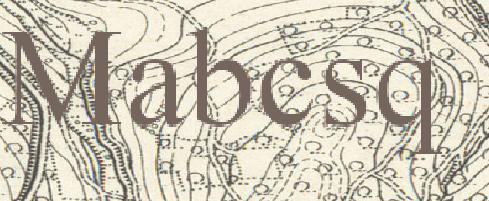
\includegraphics[width = 0.9\linewidth]{img/Mabcsq.jpg}
    \caption{Beispiel für künstlich erzeugte Daten\label{daten:daten:beispiele}}
\end{figure}

\subsection{Bilderkennung}
\label{daten:bilderkennung}

Die mit dem Datengenerator erzeugten Bilder werden vor der Eingabe in das Netzwerk zunächst auf eine einheitliche
Größe (Breite: Wortlänge $L$ multipliziert mit 32, Höhe 64) skaliert. Anschließend werden sie in ein Graubild des
Typs \texttt{float32} umgewandelt und auf Werte zwischen 0 und 1 normalisiert.

Das Bilderkennungsverfahren folgt dem von \textit{Shi et al.}\ vorgestellten Ansatz (vgl.~\cite{shi2017}). Es wird eine
Hierarchie mehrerer miteinander verbundener \textit{convolutional layer}, \textit{max-pooling layer},
\textit{batch normalization layer} und schlussendlich eines bidirektionalen \gls{lstm} \textit{layers} erzeugt, an das
sich ein \textit{fully-connected layer} für die Buchstabenaktivierung anschließt (siehe
Tabelle~\ref{daten:bilderkennung:conv}).

Bis zu diesem Punkt entspricht das \textit{Trainings}-Netzwerk dem \textit{Inferenz}-Netzwerk.

\begin{table}
    \caption{Netzwerkkonfiguration des Bilderkennungsteils}
    \centering
    \begin{tabular}{|c|c|}
        \hline
        \textbf{Typ} & \textbf{Konfiguration}\\ \hline \hline
        Input & $(L * 32) * 64$ \textit{Grey-scale}-Bilder\\ \hline
        Convolution & 64 Filter, (3, 3)-Kernel, (1, 1)-Stride, same-Padding, relu-Aktivierung\\ \hline
        MaxPooling & (2, 2)-Fenster, (2, 2)-Stride\\ \hline
        Convolution & 128 Filter, (3, 3)-Kernel, (1, 1)-Stride, same-Padding, relu-Aktivierung\\ \hline
        MaxPooling & (2, 2)-Fenster, (2, 2)-Stride\\ \hline
        Convolution & 256 Filter, (3, 3)-Kernel, (1, 1)-Stride, same-Padding, relu-Aktivierung\\ \hline
        Convolution & 256 Filter, (3, 3)-Kernel, (1, 1)-Stride, same-Padding, relu-Aktivierung\\ \hline
        MaxPooling & (1, 2)-Fenster, (2, 2)-Stride\\ \hline
        Convolution & 512 Filter, (3, 3)-Kernel, (1, 1)-Stride, same-Padding, relu-Aktivierung\\ \hline
        BatchNormalization & - \\ \hline
        Convolution & 512 Filter, (3, 3)-Kernel, (1, 1)-Stride, same-Padding, relu-Aktivierung\\ \hline
        MaxPooling & (1, 2)-Fenster, (2, 2)-Stride\\ \hline
        Convolution & 512 Filter, (2, 2)-Kernel, (1, 1)-Stride, valid-Padding, relu-Aktivierung\\ \hline
        Reshape & - \\ \hline
        LSTM & Bidirektional, 512 Einheiten, alle Sequenzen, Vereinigung: Summe\\ \hline
        Dense & 53 Einheiten, he\_normal-Initialisierung, softmax-Aktivierung\\ \hline
    \end{tabular}
    \label{daten:bilderkennung:conv}
\end{table}

\subsection{Textklassifizierung}
\label{daten:textklassifizierung}

Im Unterschied zur Methode von \textit{Shi et al.}\ kommt für die Textklassifizierung bzw.\ -dekodierung kein spezieller
Algorithmus zum Einsatz, sondern das Verfahren des 2006 von \textit{Graves et al.}\ entwickelten \gls{ctc}.

Die \gls{ctc}-Methode wurde für die Erkennung nicht-segmentierter sequentieller Daten konzipiert. In dieser Form liegen
beispielsweise digitalisierte Handschriften, Sprach- oder Gestenaufnahmen vor, deren einzelne Sequenzschritte sich nicht
immer eindeutig voneinander abgrenzen lassen: Wann endet bei der Aussprache eines Wortes ein Buchstabe? Wann beginnt der
nächste? In Schreibschriften, die Wörter in einer einzigen Handbewegung produzieren, lassen sich Anfang und Ende
konkreter Buchstaben häufig ebenfalls nur schwierig bestimmen.

Zum Zeitpunkt der Vorstellung der \gls{ctc}-Methode war für diese Art von Aufgaben die Nutzung eines \gls{hmm} oder
\gls{crf} üblich, die jedoch erhebliches Vorwissen über das zu lösende Problem voraussetzten und die explizite
Definition von Abhängigkeiten verlangten (vgl.~\cite{graves2006}, S.~369).

Die Verwendung eines \gls{rnn} (wie etwa eines \gls{lstm}) zu diesem Zweck erfordert -- abgesehen von der Definition
der Ein- und Ausgangsformate -- kein weiteres Wissen über das Problem. \gls{rnn} eignen sich darüber hinaus gut für die
Modellierung von Sequenzen, da sie über einen internen Zustand verfügen. Die damals bekannten auf dem Gebiet des Machine
Learning verwendeten Zielfunktionen (Loss-Funktionen) mussten jedoch für jeden Punkt der Sequenz bzw.\ Zeitschritt
separat definiert werden. Dies hatte zur Folge, dass \gls{rnn} nur darauf trainiert werden konnten, voneinander gänzlich
unabhängige Klassifizierungen vorzunehmen. Die \textit{Trainings}-Daten mussten daher manuell segmentiert und die 
Ausgabe nachbearbeitet werden (vgl.~\cite{graves2006}, S.~369). 

Ein damals weit verbreiteter Ansatz bestand darin, \gls{rnn} mit \gls{hmm} zu kombinieren: \gls{hmm} können die
Sequenzen während des \textit{Trainings} automatisch segmentieren sowie die Ausgabe der \gls{rnn} verarbeiten. Dieses
\textit{hybride} System erbte jedoch die oben erwähnten Nachteile von \gls{hmm} (vgl.~\cite{graves2006}, S.~369 - 370).

Dagegen ermöglicht die \gls{ctc}-Methode die Zuordnung von \textit{Labels} zu nicht-segmentierten Eingabesequenzen.
Dadurch ist sie für Anwendungsfälle, die eine solche Segmentierung nicht brauchen (wie etwa der Erkennung von
Handschriften, bei der die Abgrenzung zwischen Buchstaben mitunter schwierig ist) besonders gut geeignet; jedoch ist sie
für Probleme, die eine solche Segmentierung voraussetzen (z.B.\ die Voraussage von Proteinstrukturen) weniger geeignet.
(vgl.~\cite{graves2006})

Im vorliegenden Problem der topographischen Karten wurde die \gls{ctc}-Methode vor allem deshalb ausgewählt, um dem
mitunter schreibschriftartigen Charakter historischer Schriftarten zu begegnen. \textit{Keras} selbst bietet keine
Implementierung der \gls{ctc}-Methode, jedoch ist sie über das \textit{TensorFlow}-Backend nutzbar.

Ab diesem Punkt besteht ein Unterschied zwischen dem \textit{Trainings}- und dem \textit{Inferenz}-Netzwerk. An den
in Abschnitt~\ref{daten:bilderkennung} beschriebenen Bildverarbeitungsteil schließt sich im \textit{Trainings}-Netzwerk
\textit{TensorFlows} \gls{ctc}-Loss-Funktion (\texttt{ctc\_batch\_cost}) an, die mittels eines \textit{Keras}-Lambdas
als eigene Schicht in das Netzwerk integriert werden kann; hier ersetzt sie die sonst über \textit{Keras} spezifizierte
Loss-Funktion (siehe Quelltext~\ref{daten:textklassifizierung:training}).

Bei der \textit{Inferenz} ist das Vorhandensein der \gls{ctc}-Loss-Funktion nicht notwendig. Stattdessen lässt sich die
Ausgabe der \gls{lstm}-Schicht mit \textit{TensorFlows} Funktion \texttt{ctc\_decode} direkt dekodieren (siehe
Quelltext~\ref{daten:textklassifizierung:inferenz}).

\begin{code}
\begin{minted}{python}
from keras import backend as K
from keras.layers import Input, Lambda
from keras.models import Model

def ctc_lambda_func(args):
    y_pred, labels, time_steps, label_length = args
    return K.ctc_batch_cost(labels, y_pred, time_steps,
                            label_length)

# Modelldefinition - Bilderkennungsanteil
# Dann:
labels       = Input(name = "labels", shape = [word_length],
                     dtype = "float32")
time_steps   = Input(name = "time_steps", shape = [1],
                     dtype = "int64")
label_length = Input(name "label_length", shape = [1],
                     dtype = "int64")

# prediction ist der letzte Dense-Layer der Bilderkennung
loss = Lambda(ctc_lambda_func, output_shape = (1, ), name = "CTC")
             ([prediction, labels, time_steps, label_length])

# CTC-Loss mit Bilderkennung kombinieren
model = Model(inputs = [input_data, labels,
                        time_steps, label_length],
              outputs = [loss])

# Loss wird in obigem Lambda berechnet -> hier nur Dummyfunktion
model.compile(loss = {"CTC": lambda y_true, y_pred: y_pred},
              optimizer = sgd, metrics = {...})

# Model kann jetzt für Training verwendet werden
\end{minted}
\captionof{listing}{Nutzung der CTC-Loss-Funktion beim \textit{Training}}
\label{daten:textklassifizierung:training}
\end{code}

\begin{code}
\begin{minted}{python}
import numpy as np

from keras import backend as K

alphabet = "ABCDEFGHIJKLMNOPQRSTUVWXYZabcdefghijklmnopqrstuvwxyz"

int_to_char = dict((i, c) for i, c in enumerate(alphabet))

def ctc_decode(y_preds):
    results = []
    y_pred_len = np.ones(y_preds.shape[0]) * y_preds.shape[1]

    # Dekodierung der LSTM-Ausgabe
    # greedy = True führt eine Best-Path-Suche durch,
    # andernfalls müsste vorher ein Wörterbuch definiert werden
    decoded, _ = K.ctc_decode(y_preds, input_length = y_pred_len,
                              greedy = True)

    # tf.keras.backend.ctc_decode gibt ein Tupel von
    # einelementigen Listen zurück. Das eine Element ist der
    # kodierte Buchstabe, die Vereinigung der Listen somit das
    # kodierte Wort.
    for label in K.get_value(decoded[0]):
        result = []
        for i in label:
            if i == -1:
                continue # überspringe blanks
            # Umwandlung von labels in Buchstaben
            result.append(int_to_char[i])
        results.append(''.join(result)) # dekodierter String
    return results

# Modelldefinition - Bilderkennungsanteil; Gewichte und Bilder
# laden. Dann:

# hier noch kodiert und mit Blanks
predictions = model.predict(images)

# hier dekodierter String
decodeds = ctc_decode(predictions)
\end{minted}
\captionof{listing}{Dekodierung im Zuge der \textit{Inferenz}}
\label{daten:textklassifizierung:inferenz}
\end{code}

\subsection{Fixe und variable Wortlängen}
\label{daten:wortlaenge}

Der in den vorherigen Abschnitten vorgestellte Netzaufbau zur Bilderkennung und Textklassifizierung ist in der
beschriebenen Form nur auf Bilder anwendbar, deren enthaltene Texte alle über die gleiche Anzahl an Buchstaben
verfügen. Da es unter Realbedingungen äußerst unwahrscheinlich ist, nur auf Orts- und Flurbezeichnungen der selben
Wortlänge zu treffen, ist die Anwendbarkeit auf unterschiedliche Wortlängen ein wichtiges Ziel. Zu diesem Zweck muss
das vorgestellte Netz an einigen im Folgenden aufgeführten Punkten geändert werden:

\begin{itemize}
    \item Die zu erkennende Wortlänge wurde auf zwei bis acht Buchstaben festgesetzt. Eine spätere Erweiterung auf
          längere Wörter ist unkompliziert möglich.
    \item Die Nutzung von \gls{lstm}-Schichten erfordert die vorherige Festsetzung der Dimensionen der eingehenden
          Daten. Die zu verarbeitenden Bilder werden deshalb auf eine Breite von 256 Pixeln und eine Höhe von 64 Pixeln
          normiert. Die Umwandlung in \texttt{float32}-Greyscale-Bilder bleibt davon unberührt.
    \item Die \gls{ctc}-Methode benötigt keine weitere Anpassung, da diese prinzipbedingt mit Sequenzen beliebiger
          Länge umgehen kann.
\end{itemize}

\subsection{Umsetzung auf dem HPC-System \textit{Taurus}}
\label{daten:taurus}

Zur Ausführung der Python-Skripte für \textit{Training} und \textit{Inferenz} auf dem zur TU Dresden gehörigen
HPC-System \textit{Taurus} ist das Laden der im Abschnitt~\ref{daten:taurus:module} genannten Module nötig. Die Nutzung
mehrerer GPUs erfordert kleinere Anpassungen am Quelltext der Skripte, die in Abschnitt~\ref{daten:taurus:multigpu}
aufgeführt werden.

\subsubsection{Verwendete Hardware}
\label{daten:taurus:hardware}

Sowohl das \textit{Training} als auch die \textit{Inferenz} wurden stets auf einem der im \textit{Taurus} vorhandenen
GPU-Knoten mit vier NVIDIA Tesla K80 und 62 GiB Arbeitsspeicher durchgeführt (Partition \texttt{gpu2}).

Der Datengenerator wurde (je nach Verfügbarkeit) auf einem der \textit{Taurus}-CPU-Knoten betrieben, in der Regel auf
einem Knoten der \texttt{sandy}-Partition mit 16 CPU-Kernen und 30\ GiB Arbeitsspeicher.

\subsubsection{Verwendete Module}
\label{daten:taurus:module}

Sowohl die \textit{Trainings}- und \textit{Inferenz}-Skripte als auch der Datengenerator wurden innerhalb der
SCS5-Umgebung verwendet.

Die Skripte für das \textit{Training} und die \textit{Inferenz} erfordern neben dem \textit{Keras}-Framework zusätzlich
die Bibliotheken \textit{NumPy} (für den Umgang mit großen Arrays) und \textit{OpenCV} (für die Bildvorverarbeitung).
Das Modulsystem des \textit{Taurus} stellt alle genannten Abhängigkeiten bereit; zusätzlich sorgt das Laden des
\textit{Keras}-Moduls dafür, dass die \textit{NumPy}-Bibliothek als Teil von Python automatisch mitgeladen wird. Für die
Ausführung genügt deshalb das Laden der \textit{Keras-} und \textit{OpenCV}-Module. Zum gegenwärtigen Zeitpunkt
(20.\ September 2018) werden \textit{Keras} in der Version \texttt{2.2.0-foss-2018a-Python-3.6.4} und \textit{OpenCV} in
der Version \texttt{3.4.1-foss-2018a-Python-3.6.4} geladen.

Der Datengenerator bringt diverse Abhängigkeiten mit sich, die durch das \textit{Taurus}-Modulsystem nicht vollständig
abgedeckt werden können. Aus diesem Grund wurde für seinen Einsatz im Rahmen des ScaDS-Projekts eine virtuelle
Python-Umgebung (\textit{venv}) angelegt, in der die benötigten Python-Pakete vorhanden sind. Diese \textit{venv} kam
auch bei der Anfertigung dieser Arbeit zum Einsatz. Sie befindet sich auf dem \textit{Taurus} im
ScaDS-Projektverzeichnis unter dem folgenden Pfad:

\texttt{/projects/p\_scads/keras/new\_venv2}
